%
% $RCSfile: core_model.tex,v $
%
% Copyright (C) 2002-2008. Christian Heller.
%
% Permission is granted to copy, distribute and/or modify this document
% under the terms of the GNU Free Documentation License, Version 1.1 or
% any later version published by the Free Software Foundation; with no
% Invariant Sections, with no Front-Cover Texts and with no Back-Cover
% Texts. A copy of the license is included in the section entitled
% "GNU Free Documentation License".
%
% http://www.cybop.net
% - Cybernetics Oriented Programming -
%
% http://www.resmedicinae.org
% - Information in Medicine -
%
% Version: $Revision: 1.1 $ $Date: 2008-08-19 20:41:06 $ $Author: christian $
% Authors: Christian Heller <christian.heller@tuxtax.de>
%

\subsection{Core Model}
\label{core_model_heading}
\index{Res Medicinae Core Model}
\index{Electronic Health Record as Core Model}

Many kinds of application modules are needed in a healthcare-specific
\emph{Information Technology} (IT) environment. The tasks they fulfill,
together with a proposed name within the \emph{Res Medicinae} project, are
listed following:

\begin{itemize}
    \item[-] \emph{Revue:} Portal for module starting
    \item[-] \emph{Residenz:} Administrative data management
    \item[-] \emph{Record:} Clinical documentation
    \item[-] \emph{Rezept:} Prescription ordering and management
    \item[-] \emph{Reform:} Form printing
    \item[-] \emph{Report:} Public health reporting and tracking
    \item[-] \emph{Reagenz:} Laboratory- and test result retrieval
    \item[-] \emph{Rendezvous:} Scheduling
    \item[-] \emph{Roentgen:} Clinical imaging
    \item[-] \emph{Rechnung:} Billing
    \item[-] \emph{Richtig:} Statistics
    \item[-] \emph{Register:} Pharmaceutical reference
    \item[-] \emph{Ratlos:} Lexicon-, terminology- and code set query
\end{itemize}

\begin{figure}[ht]
    \begin{center}
        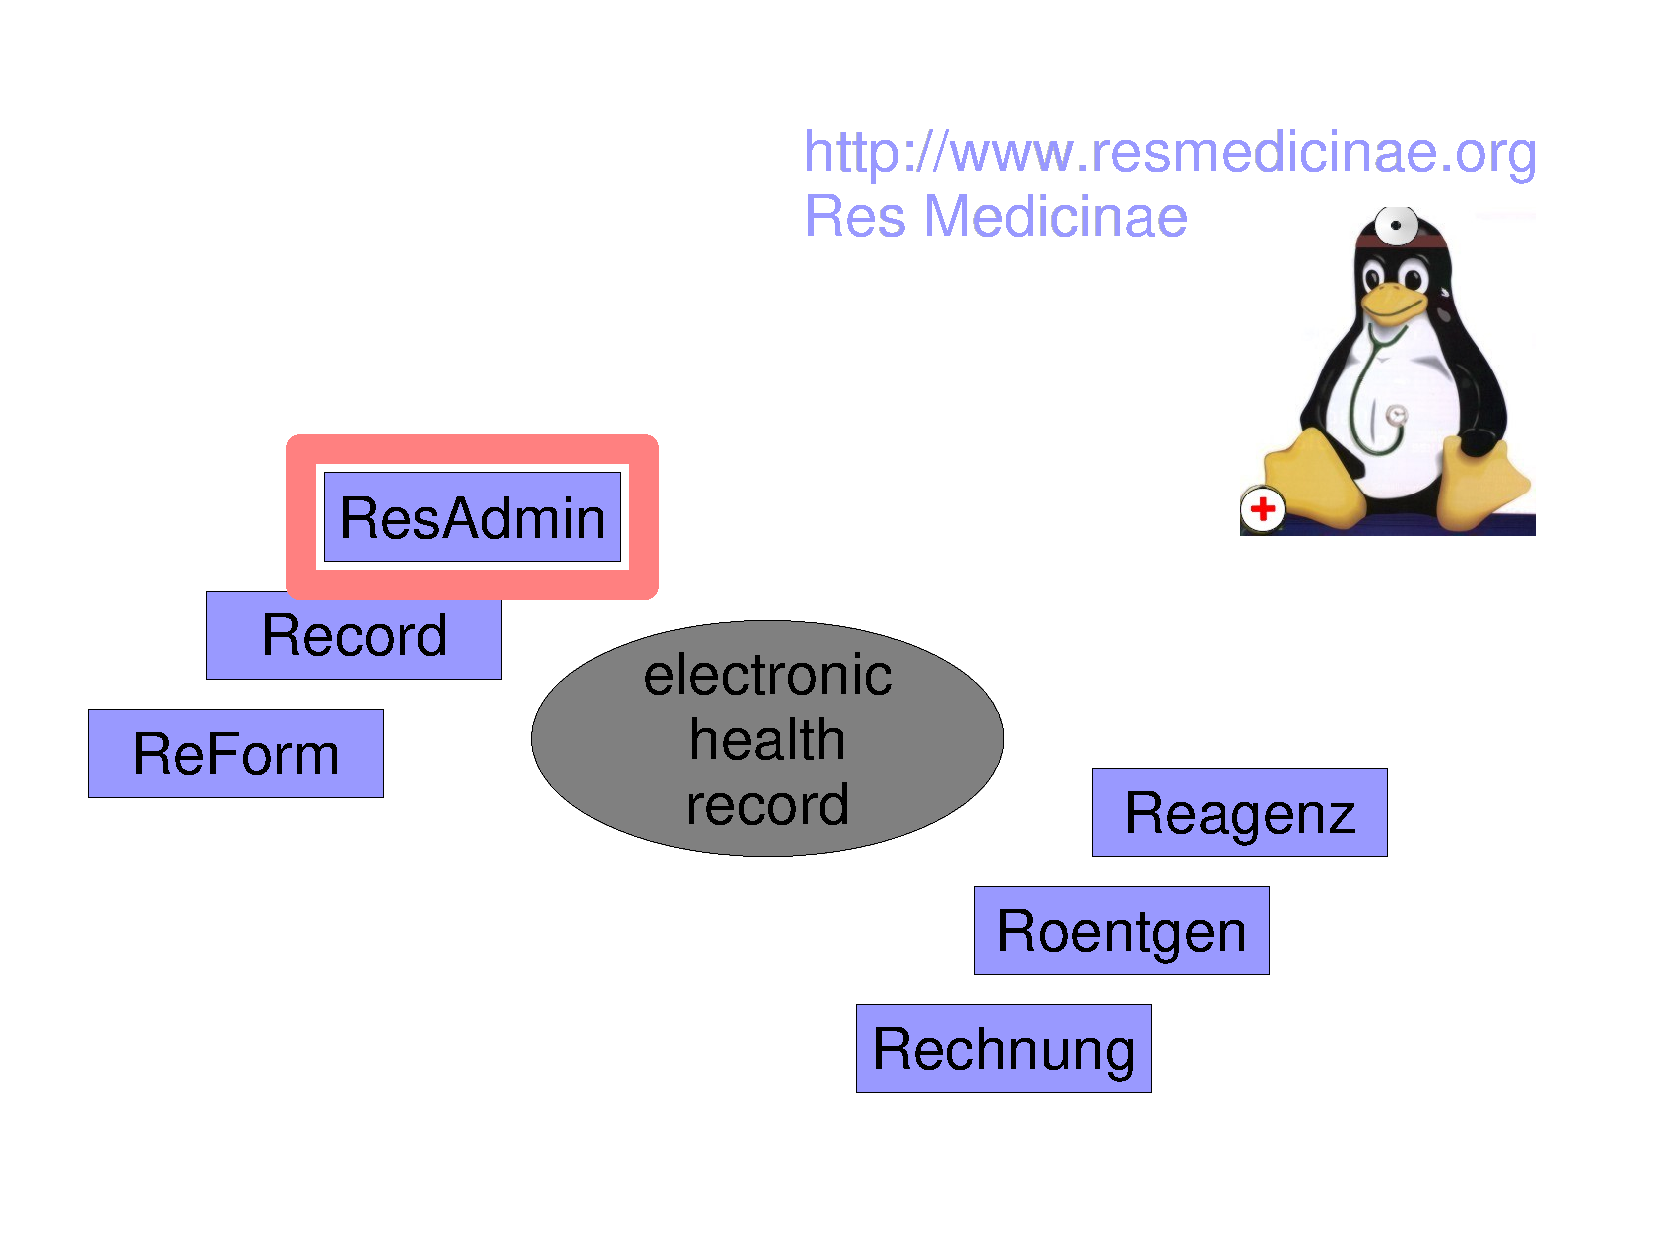
\includegraphics[scale=0.3,angle=-90]{graphic/core.pdf}
        \caption{Applications Grouped around an Electronic Health Record Core}
        \label{core_figure}
    \end{center}
\end{figure}

Figure \ref{core_figure} shows some of these modules, together with an EHR as
their central data structure.
